\documentclass{article}
\usepackage[utf8]{inputenc}
\usepackage{graphicx}
% RENAME FILE TO 910995.pdf when I submit.

% change reference style to [1], remove stupid sorting, language changed so date in ddmmyyyy
\usepackage[backend=biber, style=numeric, sorting=none, language=australian]{biblatex}
\addbibresource{References.bib}

\title{Detecting User Engagement Using \\ Mouse Tracking Data:\\
    \large Project Specification
}
\author{David Saunders (910995)}
\date{April 2020}

\begin{document}
\maketitle

\begin{abstract} 
    This project specification reviews relevant materials and the background of my project.
    The motivation and aims of the project are explained, and a comprehensive plan of work for the summer is present.
    
\end{abstract}

\tableofcontents

% \section*{Mark scheme}
% This coursework contributes 50\% of the mark for the module. The size is
% approximately 5000 words (excluding references) – due on Wednesday 29
% April 2020 (11:00 am).

% This report should give a literature review over your project and describe
% any background research that you have carried out. 
% You should state the motivation and aims of the project. 
% It should include a complete specification of your project. 
% It should describe the project clearly and the components
% of the work which need to be developed. 
% An outline project plan for the summer should be included. 
% This plan should take into account the development methodology being used. 
% You should provide a risk analysis for the project. 
% You should view this document as providing the plan for the work
% you expect to carry out over the summer.

% Work so far if I want?
% Anticipate what people want to see.
% NOTE IN RISKS
% done initial data analysis - has certain properties.
% ANTICIPATE AUDIENCE.

% Expand on risks if I want. Probably not in table.
% LOOK OVER M10 LECTURES. CSCM10 - CSCM10 - CSCM10 - CSCM10 - CSCM10 - CSCM10 

% COnstant reevaluation, never gonna have a perfect algorithm.

% Severity and likelihood.
% 



% TO SUMMARISE The structure POINTS
% - Literature Review
%   - Background research
% - Motivation and aims of Project
%   - Clearly describe project and components 
% - Outline Project Plan
%   - Include methodology used. 
% - Risk Analysis

% • Title
% • Abstract summarising the project
% • Introduction
%       • Motivation
%       • Aims of the project
% • Background research
% • Description of the project.
%       • Including components of the work.
% • Project plan
%       • Gantt chart
%       • Risk analysis
% • Conclusion.
% • Bibliography.


% \begin{figure}[ht]
%     \centering
%     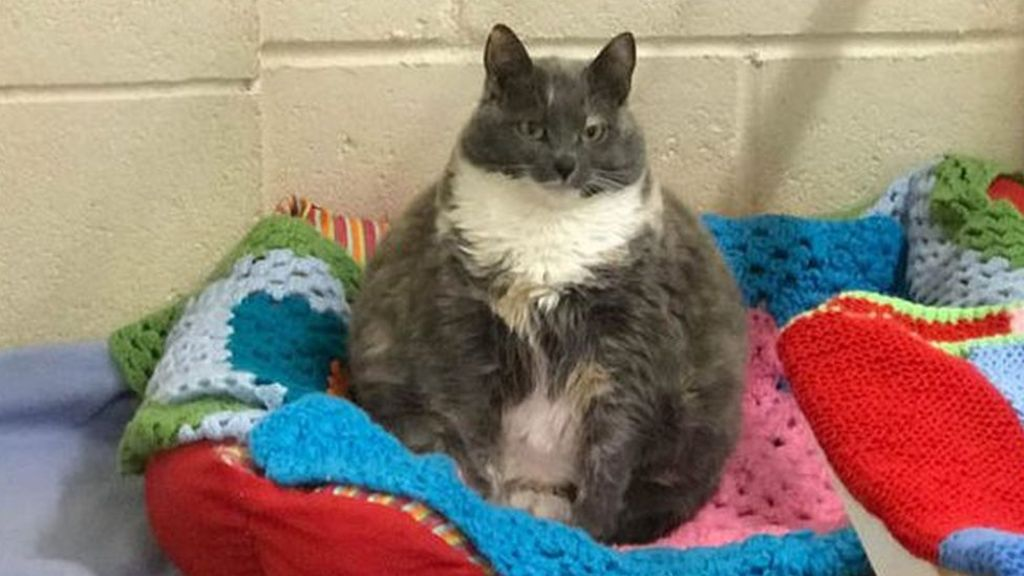
\includegraphics[scale=0.35]{Test.JPG}
%     \caption{This will be a figure showcasing some of my work}
%     \label{fig:test}
% \end{figure}
% Write section 1 here \cite{torsney2011tuner} and talk about figure \ref{fig:test}.

\section{Introduction}
%Can copy from presentation slides but fill in so they're more wordy.

% From Initial CSCM10 Report.
Crowd-sourcing marketplaces like Amazon’s Mechanical Turk are a popular service that provides a way of gathering data from real participants for studies, and human intelligence tasks \cite{paolacci2010running}. 
The level of user engagement, attention, and low quality responses can all be issues when gathering data from participants in such a distributed way \cite{ipeirotis2010quality}. 
By using data gathered from a Mechanical Turk survey and lab tests, the project is to propose methods of identifying and quantifying user engagement by using machine learning and visual analytics techniques.

\subsection{Motivation}



People are lazy. 
Often don't pay much attention 
Is there any way of measuring people's attention?

Why mouse data?
Mouse cursor position is strongly correlated with eye position. 
One paper calls it a “poor man's eye-tracker” [find]
Bulky expensive equipment for eye tracking is expensive and very obtrusive.
Hawthorn / observer effect - People react differently when being observed. 
Less obtrusive mouse tracking can make people feel less tracked and act more naturally. % goecks2000learning talks about unobtrusively observing people. CITE/TALK ABOUT 
Could even not tell them (legal ethical repercussions)!

\subsection{Aims of project}

The aims of what I want to achieve in the project will be as follows:
\begin{itemize}
    \item Visualise, analyse and understand the data.
    \item Use the data to train machine learning models to classify users between two groups.
    \item Combine the data and methods from the study data with other datasets to create a more robust model.
    \item Stretch goal? Test methods and models developed with other applications?
\end{itemize}

% Talk here about how I will achieve each aim, then describe the components of the project that I will need to complete.
% Try and link each component of the project to an aim.

% Machine learning methods
%     SVM
%     Natural Language Processing
%     N-Grams
%     LSTM Neural Networks
%     Markov models
% Deal with Imbalances in classes
%     Sampling
%     Oversampling, Undersampling
% Other mouse data sources




Applications
A good system developed could be used for other tasks to monitor attention - E.g. Survey Monika made us do. Not just for joes ice-cream
Have to decide on the trade off between a good narrow (is this the right word) classifier between attention or not and a more generalised model that can work on any task.
What I mean by that is I can model the html elements / sliders to see how users interacted to see the stock prices, or I can generalise to any such task involving mouse data.


\section{Background Research}
Anything I've looked at with help for mouse data classification algorithms? 

%\section{Literature review}
In this section I will review the literature on how to monitor attention.
%This can pretty much be the review I did for the first assignment. 

\subsection{User attention and characteristic.}


\subsection{Eye tracking}
% Copppied straight from CSCM10 Initial Report
% TODO: Refernce with Bibtex

As mentioned previously in the report non-verbal information can be used to detect a
user’s level of engagement, eye tracking is a prime example of this \cite{lala2017detection}.
Vision is one of the most powerful human senses so it may give a good measure of user engagement. 
The methodology of eye tracking is that we move our eyes to focus on particular areas that we want to see in more detail, and divert our attention to that area \cite{duchowski2007eye}. 
% duchowski2007eye is a VERY important piece of literature for the field, over 4000 citations
Thus tracking a user’s gaze can provide insight into which part of a system they’re engaged with, and how much so.

\begin{figure}[ht]
    \centering
    \centerline{
        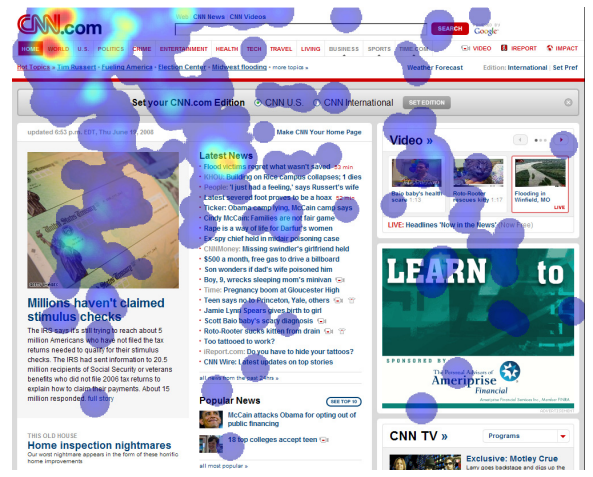
\includegraphics[scale=0.7]{EyeHeatmap.PNG}
    }
    \caption{Heatmap showing the popular locations of users eyes on a webpage CITE.}
    \label{fig:eyetrack}
\end{figure}

Eye tracking data can be used to show user interface elements that users focus their attention on as shown in Fig \ref{fig:eyetrack}. 
From this researchers were able to predict the amount of attention elements of the page would receive. 
By observing what parts of an interface users are interacting with we can determine what a user is engaging with \cite{buscher2009you}.
Eye-tracking has been used, and found success novel applications such as recording the engagement of users when playing a game. 
Tracking users eye movements helped game designers understand how users can recognise interactable game objects and could be used to investigate problematic game design issues \cite{renshaw2009towards}.

\subsection{Mouse cursor tracking}
% Copppied straight from CSCM10 Initial Report
% TODO: Refernce with Bibtex
Mouse cursor tracking
Eye tracking has historically had its limitations. 
To track subjects eyes with a good degree of accuracy required the use of expensive, intrusive equipment that frequently needed recalibrating \cite{richardson2004eye}. 
In contrast mouse movement data can be collected without the drawbacks of eye tracking and with more automatic methods, meaning more data can be collected, and on a larger scale \cite{demvsar2017quantifying}.
Research has also found that there is a correlation between a user’s gaze and their cursor position. 
The position can be considered a ``poor man’s eye tracker'' as it has been found that eye gaze match mouse position 69\% of the time \cite{cooke2006mouse}. 
Therefore it can be said that mouse data can be used as a good alternative to eye tracking data.

Mouse activity can be used as input to a neural network and output a quantifiable level of activity for a webpage. 
By using mouse data it is possible to unobtrusively record a user’s normal use of a web browser without disturbing their experience \cite{goecks2000learning}.
% Above paper touches on one of the big advantages of measuring user engagement from mouse data, it is unobtrusive! We can monitior them in the background 
It has also been found that users tend to follow the text they’re reading with the mouse cursor \cite{liu2007detecting}, and similarly scientists were able to determine what paragraph of a page was being read with an accuracy of 79\% by using mouse cursor data \cite{hauger2011using}. 
Methodologies mentioned above explore ways of classifying user engagement from eye and cursor data, however it is also possible to predict users attention and user frustration in complex webpages \cite{navalpakkam2012mouse}.
In contrast to the above literature some studies disagree that mouse cursor is always a good approximation for eye data. 
Hauger et al found that distinct cursor behaviour exists depending on the task, and that the relationship between eye gaze and mouse position is more nuanced than measuring only mouse data \cite{huang2012user}.

\subsection{Machine learning techniques???}
I've given a high level overview of the existing literature, here I will be more indepth as to the algorithms and techniques relevant to this project.




\section{Description of the project}

\subsection{Components of project}
Each of the following are separate sections that can be completed separately, but linearly.

Repeat this process N times
(
Research of different algorithms and methods.
Coding section.
The visualisations of results.
Write up of results.
)

Compile results together into dissertation.

TODO: Look at the dissertation outline so I know what stuff needs to be included so I can mention it here.

\section{Project plan}
% Look into different software methodologies
% http://www.cs.swan.ac.uk/~csetzer/articles/researchMethodologiesInComputerScience.pdf
% 

The different components of the work have been explained above.
This section will specify the timeframe and order in which the modules will be carried out.

I will be using an agile methodology as it will allow flexibility of my project and the iterative nature should help me to constantly improve it \cite{beck2001manifesto}. 

Scrum will be used as the short scrum periods will encourage bursts of development over the long summer period.

\subsection{Development methodology}
%Discuss software life cycle methodologies with Jacques.
An agile methodology such as scrum would probably be best but am I constrained  by this specification document?

We want a methodology that has a final write up, but also has lots of iterative stuff in the middle for me to research, explore, and test new algorithms.
For that reason I will be following the Scrum software lifecycle methodology.
TODO: reference 

Figure \ref{fig:Gantt} shows the sprints I will be undertaking.
The Gantt Chart was created with the free software Gantt Project \cite{GanttProject}.
Each sprint starts with a supervisor meeting where the previous work, and the plan for the next sprint will be discussed.
There will be three sprints in total, with each sprint being a fortnight long.
Each sprint will consist of researching a method I may be able to use in my project.
Then I will spend time modifying and implementing the method so that it may be used in the context of this project.
The latter half of a sprint will consist of analysing and visualising the results of the method and writing these down roughly in the dissertation document.
For example I may come across a particular variant of an artificial neural network in my research that I believe may be useful in the project.
The sprint plan would allow me to spend time implementing this network with my data and experiment with the parameters.  


\begin{figure}[ht]
    \centering
    \centerline{
        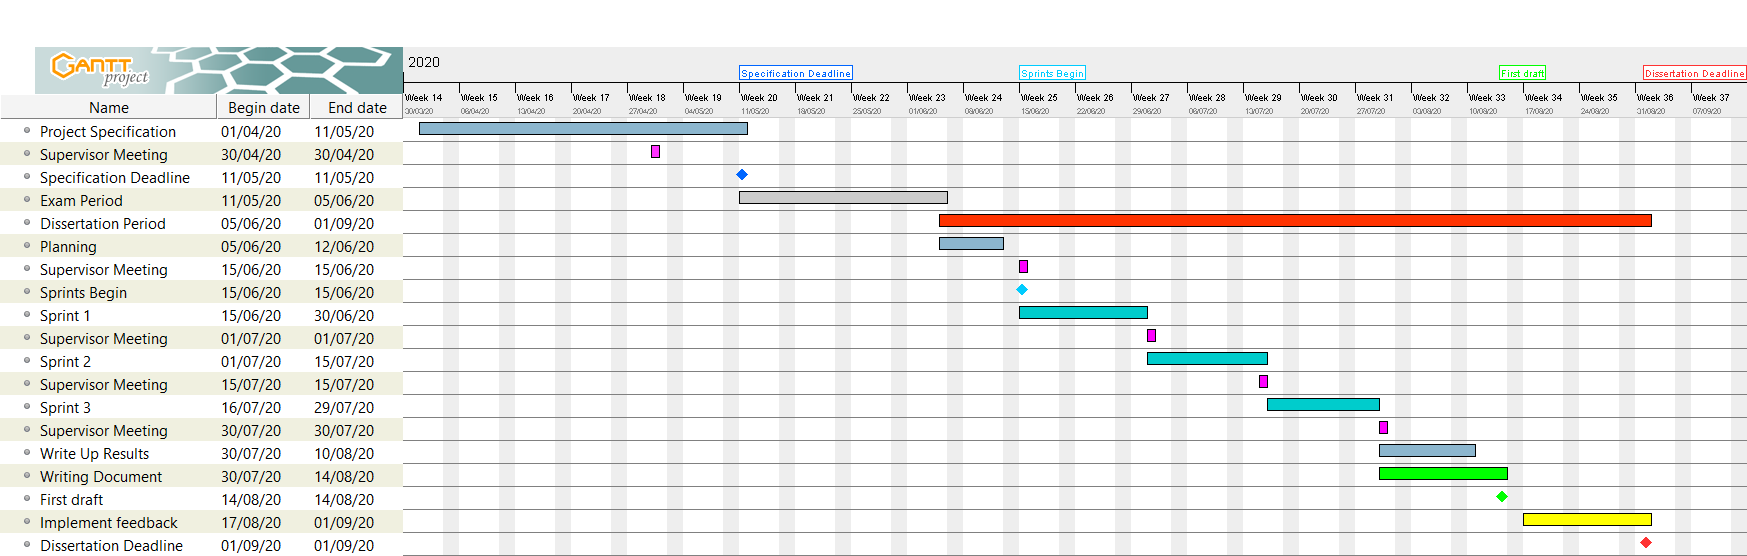
\includegraphics[scale=0.32]{GanttChart.PNG}
    }
    \caption{Gantt chart showing the planned timeline and milestones of the project.}
    \label{fig:Gantt}
\end{figure}


\subsection{Risk Analysis}
% Copy risk analysis from last year.
When creating a project there is always potential risks that the project might encounter and hinder its chances of success. 
In order to prepare and to hopefully avoid these risks I will now list and analyse the risks of my project. 
By analysing each risk individually I will be prepared in case I come across any of the potential risks and I will have developed a plan of action of what to do and how to manage myself in case of encountering them. 
Each risk is explained with the likelihood of the risk occurring and impact to the project the risk would have.
A mitigation plan is created in an attempt to prevent the risk from happening, and a contingency plan is made so I can be prepared if the risk does occur.
Below I have listed and analysed the risks and have ordered them from potentially the most dangerous to least dangerous. 


%REPLACE this table with an itemized list, like in the data visualisation module.
% - Tom said that tables can make it too restrictive.
% Just coppied from table here, make sure to flesh out later
% TODO: Flesh out risks 

% Do I keep explaination or just expand risks in the risk item?

\begin{enumerate}
    \item 
    \begin{description}
        \item[Risk:]    
        \emph{Unrealistic time plan and poor time management.}
        \item[Likelihood and Impact:]
        Medium likelihood, Medium Impact
        \item[Explaination]
        If my time is spent poorly then I could not have a piece of work finished for the submission deadline, or the work may not represent the best of my abilities.  
        \item[Mitigation:]
        Create work schedule and stick to it.
        A work schedule and plan for the summer has been created in this document which I aim to follow.
        \item[Contingency:]
        If I am unable to stick to my work schedule, I must adapt my approach to work and create an undated, more realistic schedule.
    \end{description}

    \item 
    \begin{description}
        \item[Risk:]
        \emph{Coronavirus affects me or a close family member, negatively effecting my work.}
        \item[Likelihood and Impact:]
        Medium likelihood, High Risk
        \item[Explaination]
        Coronavirus is very contagious. 
        Dispute risks it is still likely that the I may become infected. 
        \item[Mitigation:]
        Stay safe indoors during the quarantine to keep everyone safe and mitigate any risks of me catching anything.
        \item[Contingency:]
        Inform the University as soon as a situation develops so that alternative assessments can be organised.
    \end{description}

    \item 
    \begin{description}
        \item[Risk:]    
        \emph{No correlation between attention and mouse tracking data can be found.}    
        \item[Likelihood and Impact:]
        Medium likelihood, High impact
        \item[Explaination:]
        The project will involve the use of many methods to find a link between mouse tracking data and user attention.
        It is possible that after all methods have been exhausted no correlation is ever discovered, or simply doesn't exist. 
        \item[Mitigation:]
        Attempt as many different methods of classification early before writing in depth about them.  
        \item[Contingency:]
        If no insights can be gained from the given dataset, I will explore other similar datasets and attempt to find correlations there.
        I will then attempt to apply findings from other datasets to the original dataset. 
    \end{description}

    \item 
    \begin{description}
        \item[Risk:]    
        \emph{Coronavirus has a greater impact on Swansea University and  effects the available support and deadlines.}
        \item[Likelihood and Impact:]
        Low likelihood, Low impact
        \item[Explaination:]
        The virus has already shut down in person teaching and with the UK in lockdown it is unlikely the situation will become vastly different. 
        \item[Mitigation:]
        Keep informed with the University College of Science and supervisor to any news effecting the University.
        \item[Contingency:]
        TODO: What is the plan? Keep my options open? Keep updated?
        Keep updated with the situation and follow whatever advice is recommended from the university.
    \end{description}

    \item 
    \begin{description}
        \item[Risk:]    
        \item[Likelihood and Impact:]
        \item[Mitigation:]
        \item[Contingency:]
    \end{description}
\end{enumerate}

% OLD TABLE INCASE I WANT TO REVERT
% \newpage
% \begin{table}[ht]
%     \small %small not needed
%     \caption{\label{table:individual} The top association rules between individual items.}
%     \makebox[\textwidth][c]{%
%         \begin{tabular}{|p{2cm}|p{1cm}|p{1cm}|p{1cm}|p{2cm}|p{2cm}|}
%             \hline 
%             { Risk}                                                                                                       & { Probability} & { Impact} & { Combined Risk} & { Mitigation Plan}                                                                                               & { Contingency Plan}                                                                                                                  \\
%             { Unrealistic time   plan and poor time management.}                                                          & { High}        & { High}   & { High}          & { Create work   schedule and stick to it.}                                                                       & { If I am unable to   stick to my work schedule, I must adapt my approach to work and create an   undated, more realistic schedule.} \\
%             { Coronavirus affects me or a close family member, negatively effecting my work.}                           & { Medium}      & { High}   & { High}          & { Stay   safe during the quarantine to keep everyone safe and mitigate any risks of me   catching anything.}     & { Inform   the University as soon as a situation develops so we can arrange something.}                                              \\
%             { Coronavirus has a greater impact on Swansea University and  effects the available support and deadlines.} & { Medium}      & { High}   & { Medium}        & { Keep   informed with the University College of Science and supervisor to any news   effecting the University.} & { Keep my   options open? Keep updated?}                                                                                             \\
%             { No correlation between attention and mouse tracking data can be found.}                                   & { Low}         & { High}   & { Medium}        & { Attempt   as many different methods of classification early before writing in depth about   them.}             & { If no   insights can be gained from the given dataset, I will attempt to find   correlations in other datasets.}                   \\                                                                                                                    
%         \end{tabular}
%     }
% \end{table}

\section{Conclusion}

Measuring user engagement is challenging
Mouse data can help us solve that issue by showing user attention
Data Science techniques could be used to help classify the data (Not SVM)


\printbibliography

\end{document}

% Project meeting
% ############## Programming Questions ############
% Points start and end at different points, for both lab and actual, is that expected? 
%     How was it measured? Moving window?
%     How do I reference this in diss?
%     Can I just transform points to new position? But how do I do other points not just start end.

% In Data online turk has alloc-slider-5 while lab study has stuff like [id="alloc-slider-return-4"]>svg>g>circle and [id="alloc-slider-return-4"]>svg. can just remove the brackets but whats the >svg>g>circle?

% Lab has no buttons,  and some that say just html?

% Presentation Questions
% #############################################

% Marks for Presentation 65 I was happy with. Feel like 65 is good a merit but lower than other marks so should I be disappointed?

% For motivation and background of project do I just say what I did in my presentation?
% onje sentence explaion what i do why and helpful. By end of first paragraph! so people dont get lost.
% Said how I will evaluate.-  we will evalutate teh algorithm by comparing again stest dataset.

% http://pages.cs.wisc.edu/~gleicher/Web/Advice/PaperRecipe

% ##################### Project Specification #################

% No existing work section on project specificaton, so I dont say anything? Not that ive done much but transform Data and do SVM.

% Literature review for project, is this not just what I did for the initial thing? cant remember what it was called but whatever.
% - Why cant trhie approach be used for mine
% Do want to add a section maybe on NLP and semi-supervised learning. But hows NLP a literature review of project, even assuming it works at all??

% In risk assessment of project, ive said covid effecting uni, and covid effecting me. 2 more risks of me failing at time management and me failing to find any correlation between mouse and attention in the data. Is this ok?

% How would I mitigate these risks?
% I think no correlation is kinda likely, while youd intuitevly think that there may be a correlation no other studies seem to back it up and with so little data points its hard to draw any actual conclusions.


% Gantt Chart

% Whole timeline.


% - Have milesstones.
% - Sub cycles 
% - initial data analysis
% - building
% - testing
% - why didnt work
% -  evaluation 
% - repeat.

